\section{Simulation}
%%%%%%%%%%%%%%%%%%%%%%%%%%%%%

\subsection{Purpose}
The purpose of this simulation is to compare the performance of the QEKF and InEKF filters in terms of error reduction between the true and estimated state. The primary difference between these two filters is in the approach of representing rotation between different coordinate frames. In the more traditional QEKF, rotation action between states is achieved through quaternions. The InEKF utilizes a Lie group structure to represent key states. By running simulations with both filters, it can be determined whether the new Lie group-based InEKF offers advantages as compared to the quaternion based QEKF.

\subsection{Setup}
To run this comparison simulation, python scripts were created and truth trajectory data from the Mid-Air Dataset was utilized \cite{Fonder2019MidAir}.  Position, velocity, acceleration, attitude (defined as a quaternion), and angular velocity data were all sampled at a frequency of 100 Hz. For GPS measurements, the data was sampled at a rate of 1 Hz and for magnetometer measurements at 10Hz. The measurements were then emulated using the truth data, equations defined for the IMU model \eqref{eq: measurement model}, the GPS model \eqref{eq: position gps}, and the magnetometer model \eqref{eq: mag measurement model}. The standard deviations for the respective models were defined in table \eqref{tab: Measurement Noise Statistics}. The specific simulation noise statistics were choose based upon the article by John Stechschulte \cite{stechschulte2023imuspecs}. In selecting the standard deviation values, I chose values that fall between those typical of consumer-grade and industrial-grade IMUs. Note also that the random walk states are multiplied by an additional $\frac{1}{s}$ because in the error update equations the noise is multiplied by $\Delta t$.
% \begin{table}[h!]
% \centering
% \begin{tabular}{|c|c|c|}
% \hline
% \textbf{Measurement}& \textbf{Noise Standard Deviation} & \textbf{Units} \\ 
% \hline
% Accelerometer White Noise & $\sigma_{a} = 5e-3$ & $\frac{m}{s^2} \frac{1}{\sqrt{Hz}}$\\ 
% \hline
% Accelerometer Random Walk & $\sigma_{ba} = 6e-3$ & $\frac{m}{s^3} \frac{1}{\sqrt{Hz}}$\\  
% \hline
% Gyroscope White Noise & $\sigma_{\omega} = 1e-3$ & $\frac{rad}{s} \frac{1}{\sqrt{Hz}}$\\ 
% \hline
% Gyroscope Random Walk & $\sigma_{ba} = 3e-4$ & $\frac{rad}{s^2} \frac{1}{\sqrt{Hz}}$ \\ 
% \hline
% GPS White Noise & $\sigma_{\Tilde{y}_{GPS}} = 1$ & $m$ \\ 
% \hline
% Normalized Magnetometer White Noise & $\sigma_{\Tilde{y}_{Mag}} = 0.002$ & $\frac{1}{\sqrt{Hz}}$ \\ 
% \hline
% \end{tabular}
% \caption{Measurement Noise Statistics}
% \label{tab: Measurement Noise Statistics}
% \end{table}

% Notes on units
% -> To match 1 / \sqrt(Hz) for white noise need to multiple my number by \sqrt(Hz)
% -> Same needs to be done for bias. Bias is already multiplied by \Delta t so don't adjust for that
% -> Remeber units of sigma match the mean

\begin{table}[h!]
\centering
\begin{tabular}{|c|c|c|}
\hline
\textbf{Measurement}& \textbf{Noise Standard Deviation} & \textbf{Units} \\ 
\hline
Accelerometer White Noise & $\sigma_{a} = 5e-4$ & $\frac{m}{s^2}$\\ 
\hline
Accelerometer Random Walk & $\sigma_{ba} = 6e-4$ & $\frac{m}{s^3}$\\  
\hline
Gyroscope White Noise & $\sigma_{\omega} = 1e-4$ & $\frac{rad}{s}$\\ 
\hline
Gyroscope Random Walk & $\sigma_{ba} = 3e-5$ & $\frac{rad}{s^2}$ \\ 
\hline
GPS White Noise & $\sigma_{\Tilde{y}_{GPS}} = 1$ & $m$ \\ 
\hline
Normalized Magnetometer White Noise & $\sigma_{\Tilde{y}_{Mag}} = 0.05$ & $None$ \\ 
\hline
\end{tabular}
\caption{Measurement Noise Statistics}
\label{tab: Measurement Noise Statistics}
\end{table}

With the measurement data generated, a Monte Carlo simulation of 50 trials was run for each filter using the same flight trajectory. For these simulations, trajectory 2 from the Mid-Air Dataset was used which didn't lack dynamics within the trajectory. In each trial, the noise statistics and initial covariance were constant. The initial condition of each of the states were then randomized over a uniform distribution. The randomized initial states are defined below in table \eqref{tab: Initial State Variations}. Note that once the initial attitude is randomized it is converted into a initial quaternion for the QEKF and the quaternion is converted into a initial rotation matrix for the InEKF.

\begin{table}[H]
\centering
\begin{tabular}{|c|c|c|}
\hline
\textbf{Initial State} & \textbf{Randomization} & \textbf{Units} \\ 
\hline
Position  & $\mathcal{U}(p_0, 15) $ & $m$ \\ 
\hline
Velocity & $\mathcal{U}(v_0, 5)$ & $\frac{m}{s}$ \\ 
\hline
Attitude & $\mathcal{U}(\theta_0, 15)$ & $deg$\\ 
\hline
Accelerometer Bias & $\mathcal{U}(b^{a}_0, 5e-5)$ & $\frac{m}{s^3}$\\ 
\hline
Gyroscope Bias & $\mathcal{U}(b^{\omega}_0, 5e-6)$ & $\frac{rad}{s^2}$\\ 
\hline
\end{tabular}
\caption{Initial States Randomization using the Uniform Distribution}
\label{tab: Initial State Variations}
\end{table}


\subsection{Results}

The position, velocity, and attitude states were tracked across each Monte Carlo for comparison between the QEKF and InEKF filters. The truth was plotted in black against the fifty different Monte Carlo runs. Additionally, the mean and max error across the Monte Carlo trials were computed and saved in table \eqref{tab: error metrics}.

\begin{figure}[H]
    \centering
    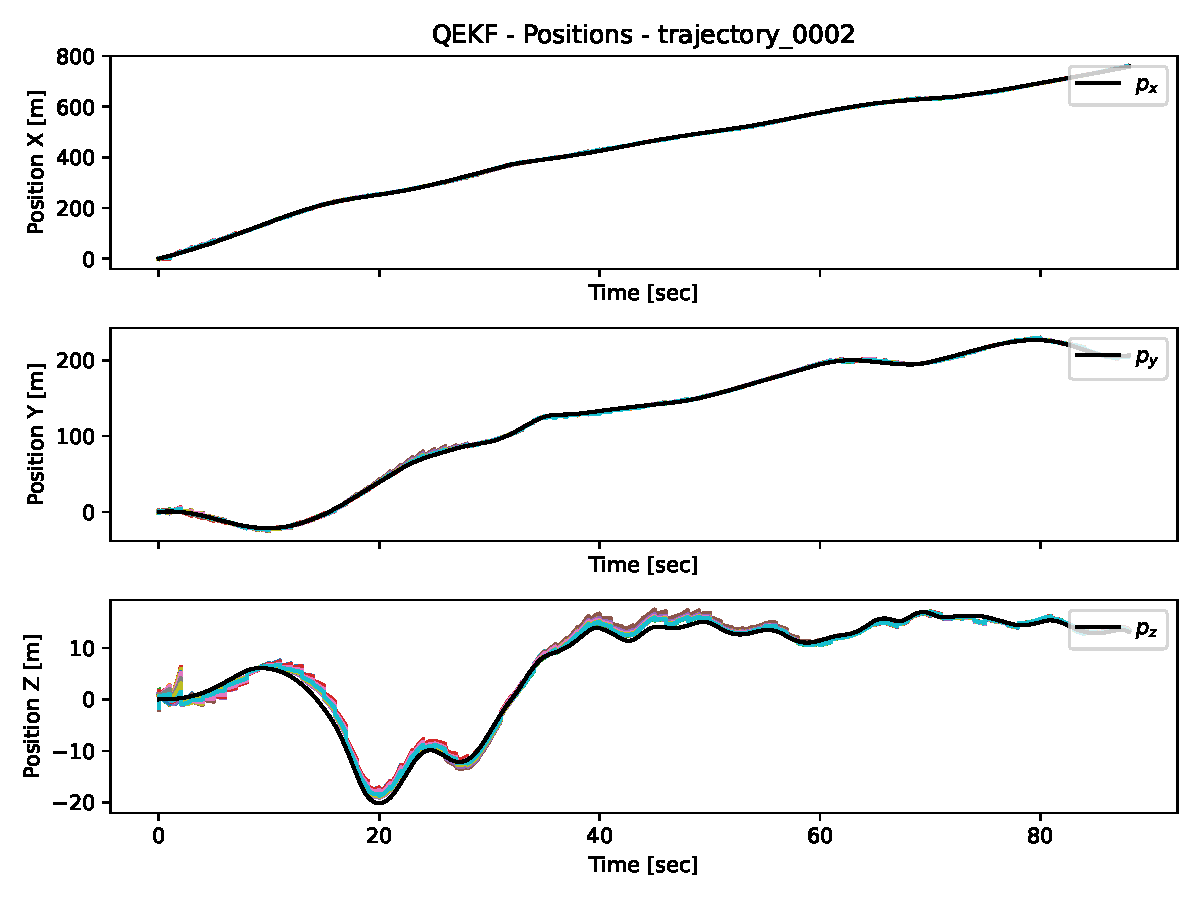
\includegraphics[width=0.8\textwidth]{figs/QEKF_trajectory_0002_positions.pdf}
    \caption{QEKF Position Monte Carlo Trials}
    \label{fig: QEKF Position Monte Carlo Trials}
\end{figure}

\begin{figure}[H]
    \centering
    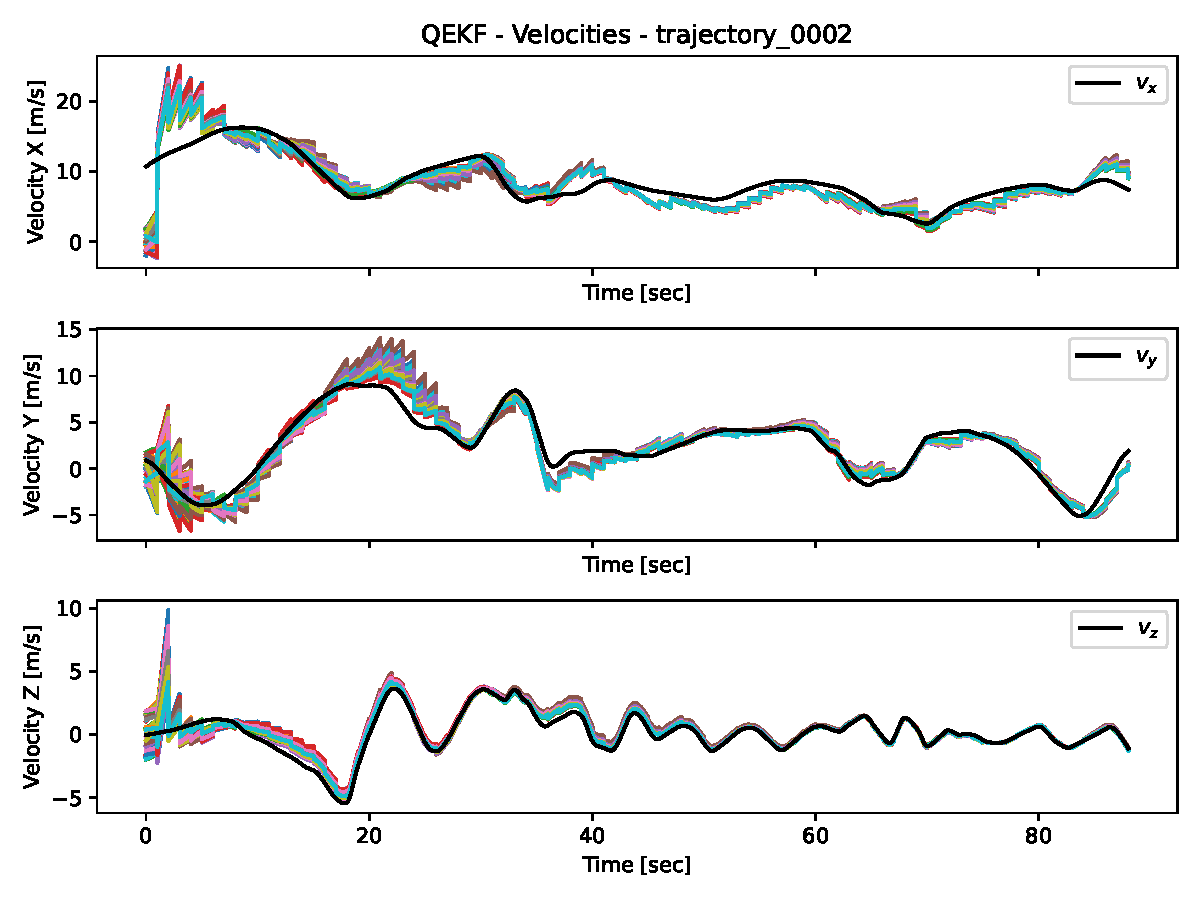
\includegraphics[width=0.8\textwidth]{figs/QEKF_trajectory_0002_velocities.pdf}
    \caption{QEKF Velocity Monte Carlo Trials}
    \label{fig: QEKF Velocity Monte Carlo Trials}
\end{figure}

\begin{figure}[H]
    \centering
    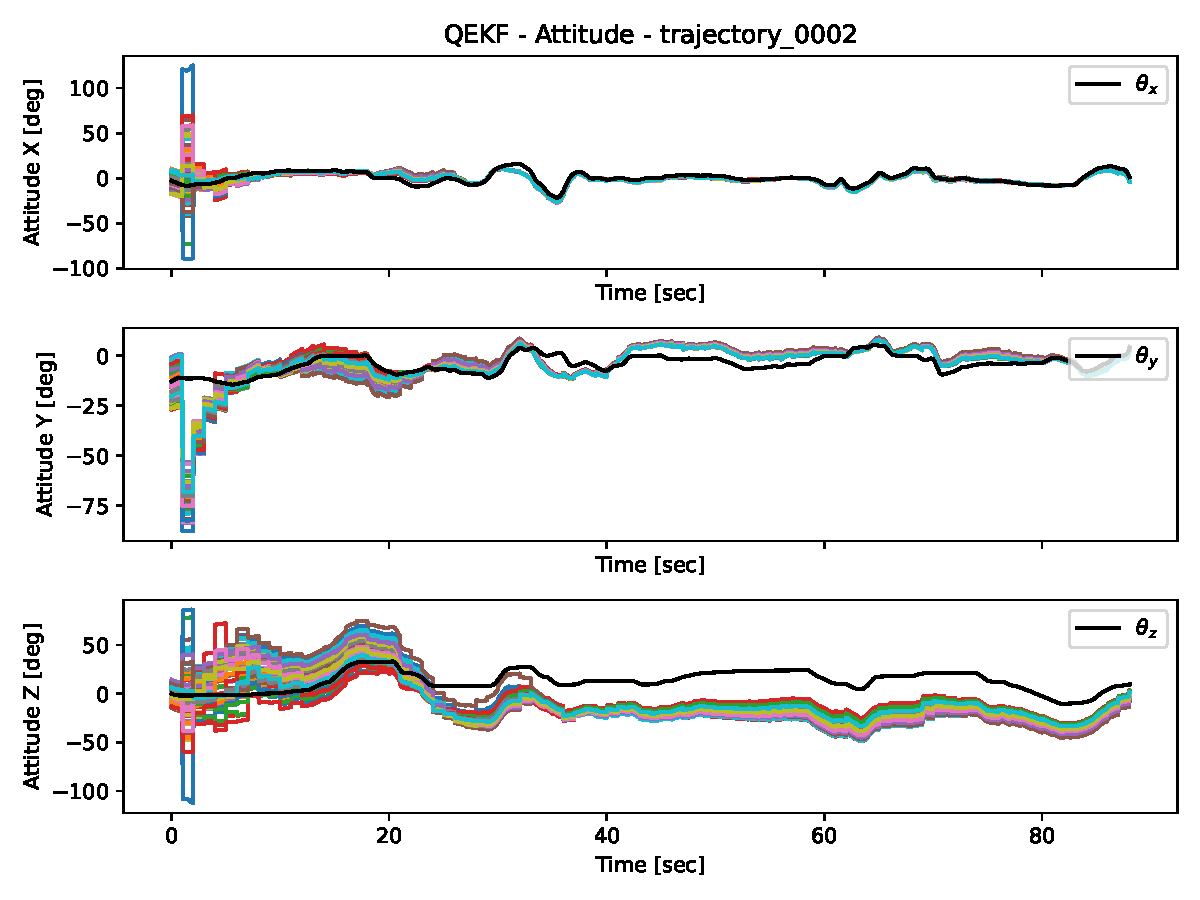
\includegraphics[width=0.8\textwidth]{figs/QEKF_trajectory_0002_attitudes.pdf}
    \caption{QEKF Attitude Monte Carlo Trials}
    \label{fig: QEKF Attitude Monte Carlo Trials}
\end{figure}

\begin{figure}[H]
    \centering
    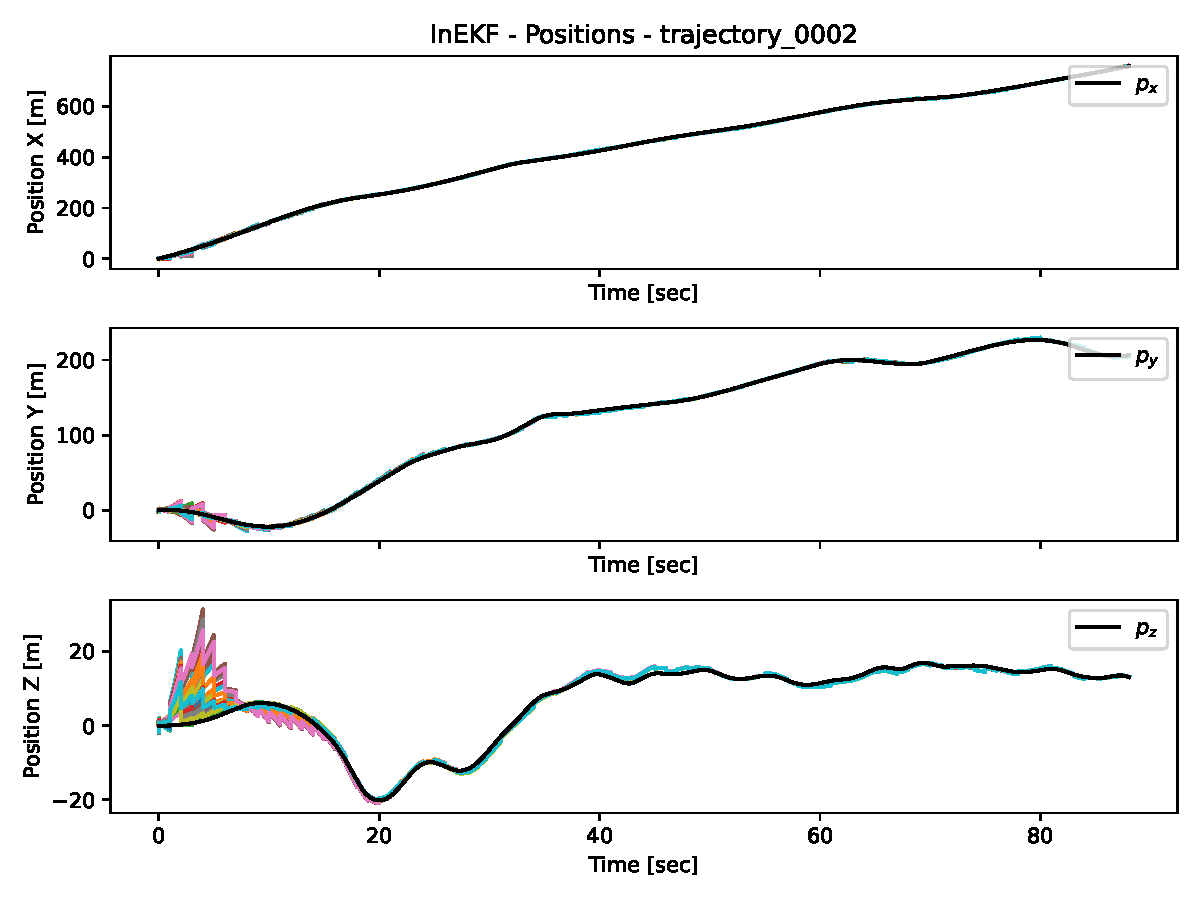
\includegraphics[width=0.8\textwidth]{figs/InEKF_trajectory_0002_positions.pdf}
    \caption{InEKF Position Monte Carlo Trials}
    \label{fig: InEKF Position Monte Carlo Trials}
\end{figure}

\begin{figure}[H]
    \centering
    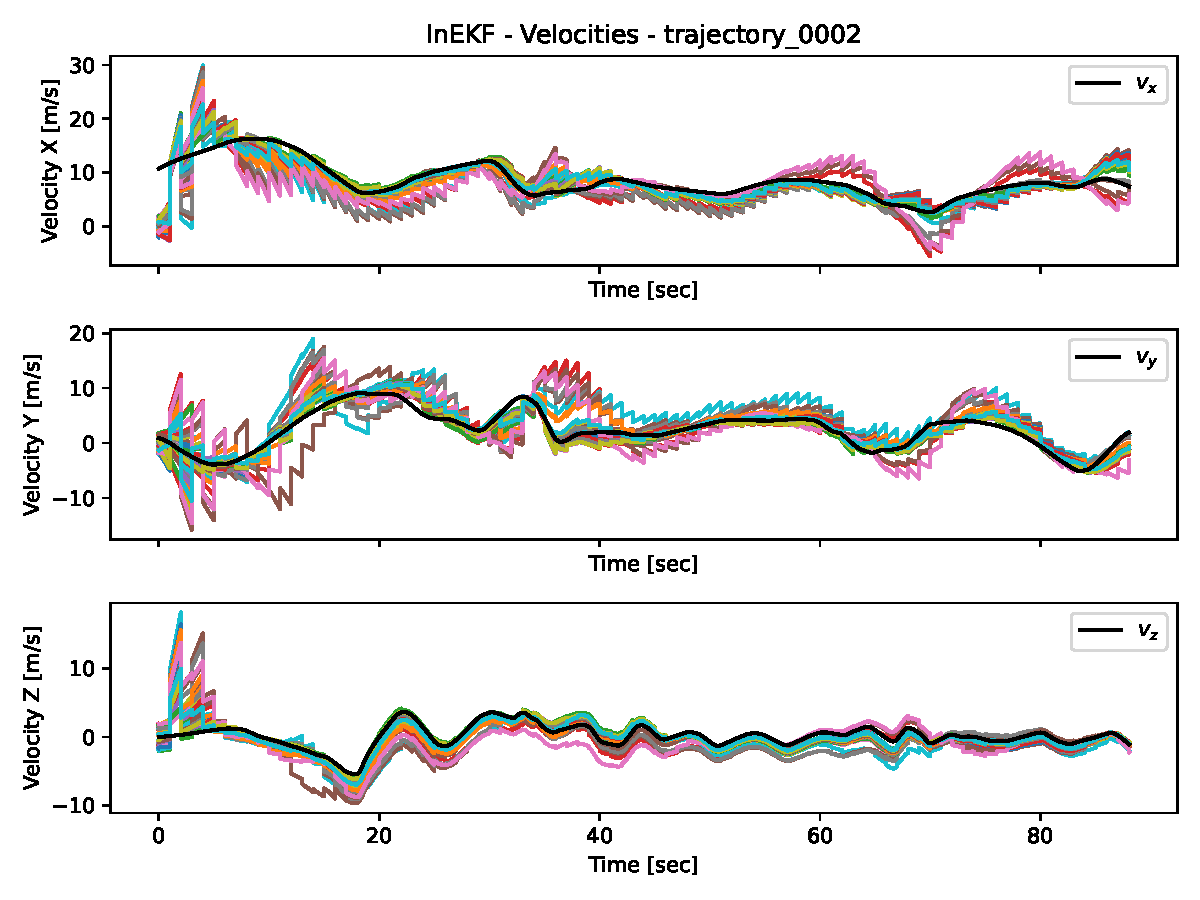
\includegraphics[width=0.8\textwidth]{figs/InEKF_trajectory_0002_velocities.pdf}
    \caption{InEKF Velocity Monte Carlo Trials}
    \label{fig: InEKF Velocity Monte Carlo Trials}
\end{figure}

\begin{figure}[H]
    \centering
    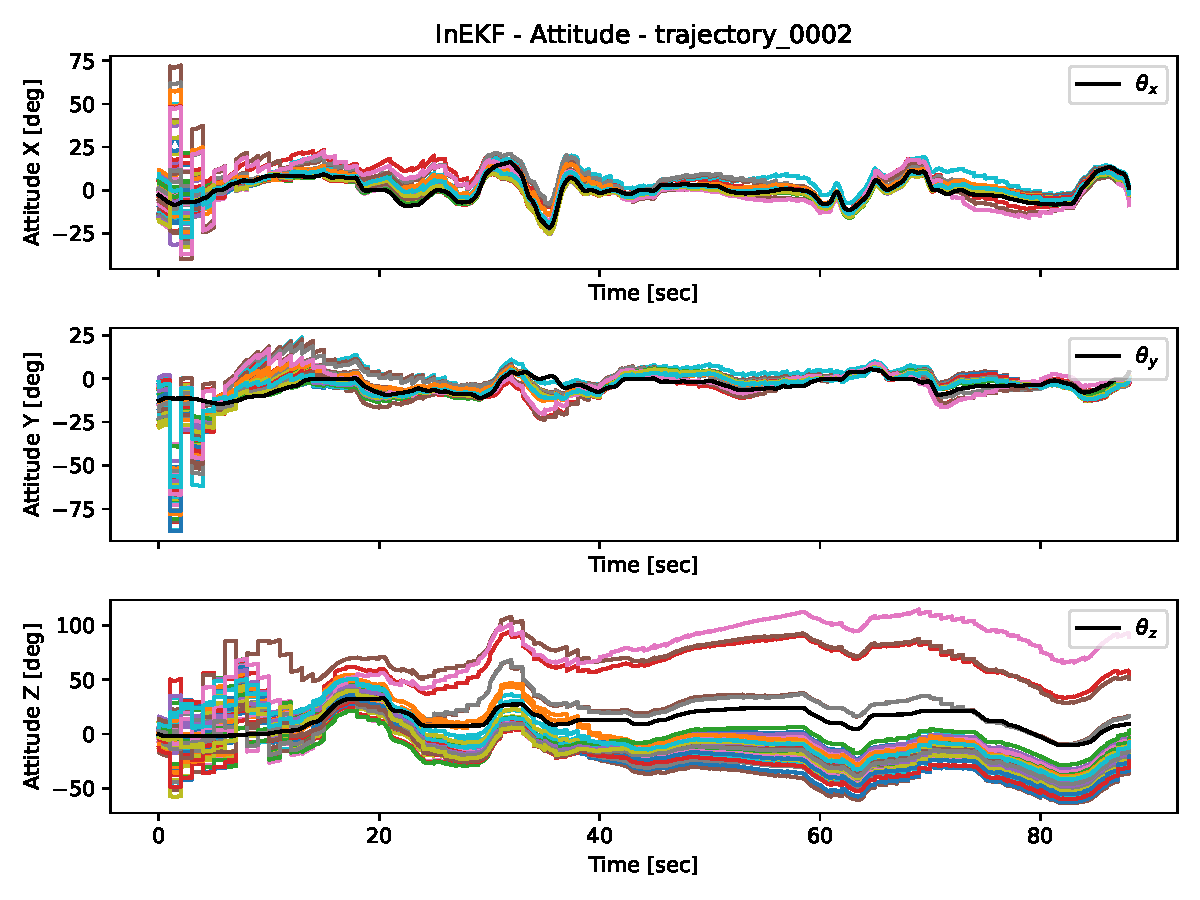
\includegraphics[width=0.8\textwidth]{figs/InEKF_trajectory_0002_attitudes.pdf}
    \caption{InEKF Attitude Monte Carlo Trials}
    \label{fig: InEKF Attitude Monte Carlo Trials}
\end{figure}

\begin{table}[H]
\centering
\begin{tabular}{|c|c|c|c|c|c|}
    \hline
    \textbf{States} & \multicolumn{4}{|c|}{\textbf{Error Metrics}} & \textbf{Units} \\
    \cline{2-5}
    & \textbf{Mean QEKF} & \textbf{Mean InEKF} & \textbf{Max QEKF} & \textbf{Max InEKF} & \\
    \hline
    Position X & 1.6605 & 1.6585 & 8.3048 & 8.5558 & $m$ \\
    Position Y & 1.0932 & 1.1037 & 6.9836 & 6.8959 & $m$ \\
    Position Z & 0.6652 & 0.6892 & 2.4909 & 2.1326 & $m$ \\
    \hline
    Velocity X & 1.1077 & 1.1209 & 4.4324 & 4.5121 & $\frac{m}{s}$ \\
    Velocity Y & 0.8094 & 0.8263 & 4.4657 & 4.4565 & $\frac{m}{s}$ \\
    Velocity Z & 0.2235 & 0.2266 & 0.8441 & 0.8191 & $\frac{m}{s}$ \\
    \hline
    Attitude X & 2.0622 & 2.0376 & 9.8943 & 10.2416 & $deg$ \\
    Attitude Y & 2.3640 & 2.3387 & 11.2028 & 11.3782 & $deg$ \\
    Attitude Z & 2.9810 & 2.8385 & 7.6830 & 7.3538 & $deg$ \\
    \hline
\end{tabular}
\caption{Monte Carlo Error Metrics for QEKF and InEKF Filters}
\label{tab: error metrics}
\end{table}

For the same simulation, plots were created to show the initial convergence of the state estimates across the different Monte Carlos. These plots only show the first ten seconds of data for the two filters such that it is visually  easier to compare when the Monte Carlo runs converged.

\begin{figure}[H]
    \centering
    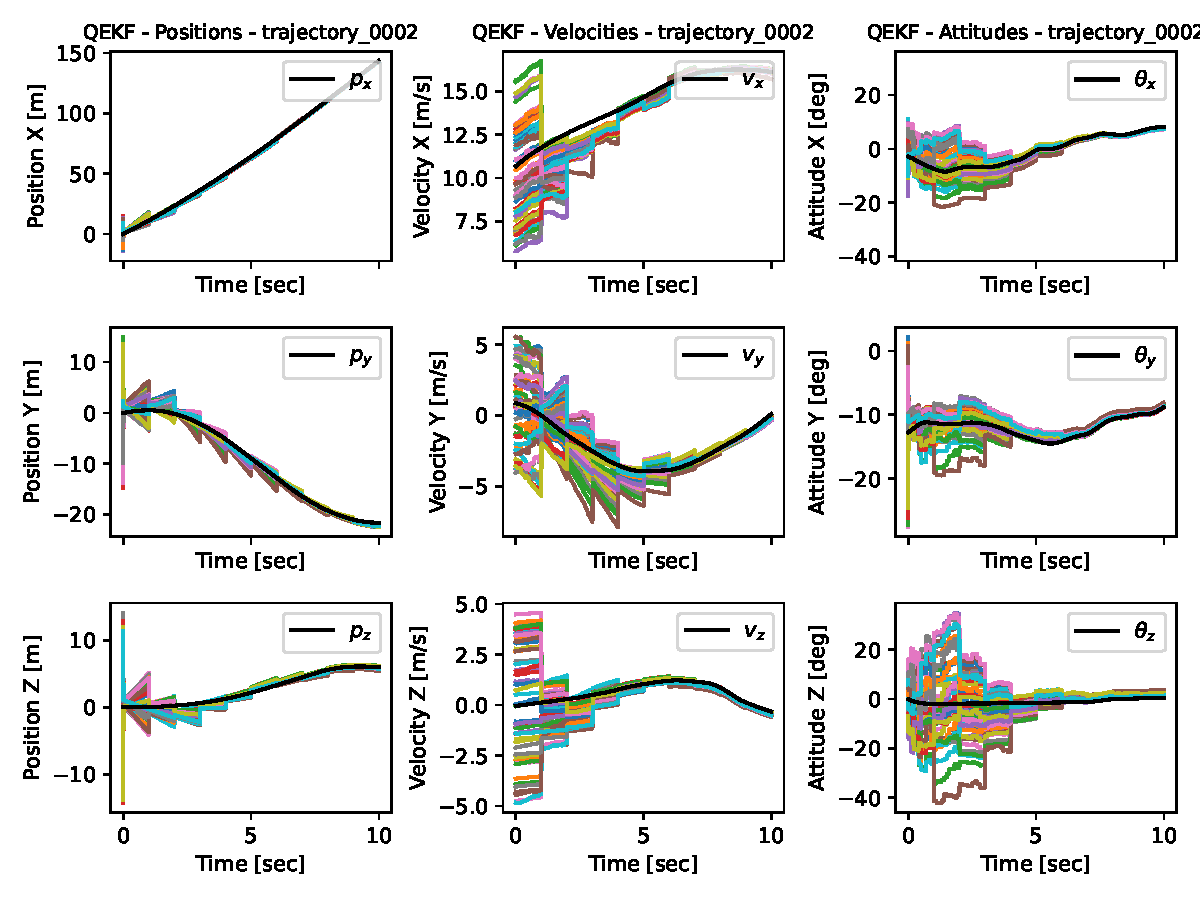
\includegraphics[width=0.8\textwidth]{figs/QEKF_trajectory_0002_initial_time.pdf}
    \caption{QEKF State Estimate Convergence Over First 10 Seconds}
    \label{fig: QEKF Convergence}
\end{figure}

\begin{figure}[H]
    \centering
    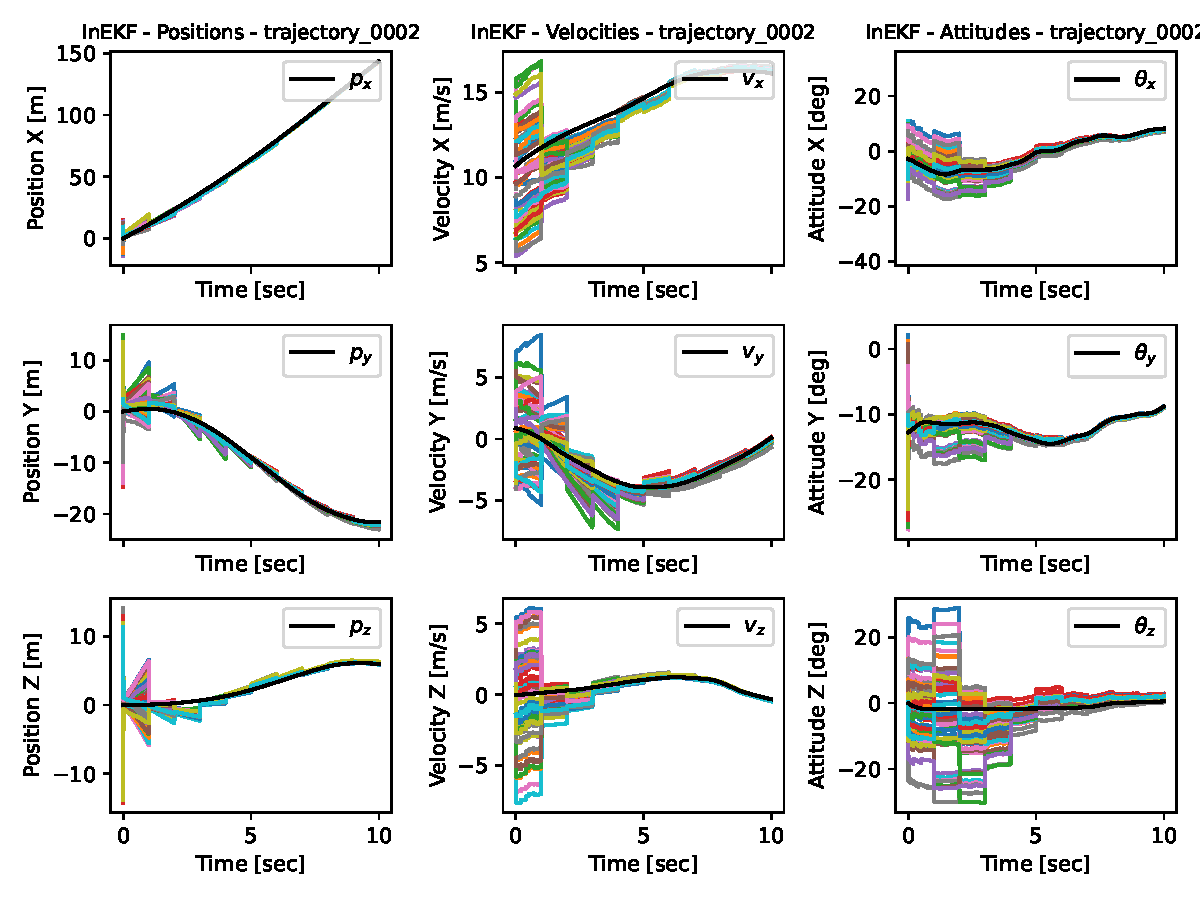
\includegraphics[width=0.8\textwidth]{figs/InEKF_trajectory_0002_initial_time.pdf}
    \caption{InEKF State Estimate Convergence Over First 10 Seconds}
    \label{fig: InEKF Convergence}
\end{figure}

\subsection{Discussion}
The purpose of these simulations was to in part determine how well the InEKF performed compared to the more standard QEKF filter. Overall, the results when comparing performance across the entire trajectory results were fairly similar. There was no state that had a significant difference between the two filters based upon the mean and max errors recorded in table \eqref{tab: error metrics}. In both filters, the velocity and attitudes are shown to have some drift in the estimate. This is in part due to the bias estimates drifting over time caused by lack of observability in these states. However, by including both GPS and magnetometer measurements observability has been improved. Previously, only GPS measurements were used. With just GPS, the Z attitude could drift with a mean error for both filters around 19 [deg]. Therefore, the 3 [deg] mean error in the Z attitude is a improvement due to the additional magnetometer measurement.

In other papers such as \cite{Contact-Aided_Invarant_EKF} and \cite{9444664}, quicker convergence of the state estimate for the InEKF was found. This can be partially seen in the results from these simulations, mainly for the velocity and attitude plots shown in figures \eqref{fig: QEKF Convergence} and \eqref{fig: InEKF Convergence}. Looking at the Z attitude, the QEKF filter has larger and more deviations in the first 5 seconds then the InEKF. Better convergence for the InEKF can also be seen in the Z velocity which has a slightly more converged state estimate closer to the truth compared to the QEKF. Overall, these convergence results, while partially existing, are not as clear as in other papers. The reason to expect a quicker convergence is that the Lie group representation offers a more accurate linearization by coupling rotation, velocity, and position. Unlike the QEKF, which treats these components independently. Despite the advantages of the Lie group representation in the InEKF, the InEKF did need to be linearized around the current state just like the QEKF due to the bias states. Therefore, having a bad initialization of the state does affect the filter because its error is no longer invariant. Another issue with the InEKF is having to switch between the right and left InEKF filters for the GPS update which is not exact for the bias augmented system. While exact when just estimating the state defined for the Lie group \eqref{eq: SE3_2 group}, the inclusion the parameter bias vector means that each switch from the right error to left then back to right creates additional error. 
 

% Using just the GPS position measurement, it is clear that both QEKF and InEKF suffer from unobservability. This affects the bias states (not shown) and causes certain states such as the attitude in the Z direction to incur large errors. By adding more measurements, observability can be improved and this issues can be reduced.

% Despite this issue, the QEKF and InEKF results can still be compared. In the InEKF plots, it is clear that quicker convergence of the states to a solution does occur which was also found in \cite{Contact-Aided_Invarant_EKF} and \cite{9444664}. This can be most clearly seen the in the velocity and attitude plots. This is due to the InEKF linearization being more accurate and being less sensitive to the initial errors as compared to the QEKF. Comparing the mean errors, the InEKF performs slightly better than the QEKF in all states besides in the Z velocity. This provides stronger evidence that the Lie group representation enhances performance by offering a more accurate linearization and by coupling rotation, velocity, and position. Unlike the QEKF, which treats these components independently, the InEKF’s approach enables a more precise representation of the system’s dynamics. Overall, the differences between the two filters were minor when using only GPS measurements. However, initial results suggest that the InEKF may hold an advantage over the QEKF. Future work incorporating additional measurements into the system will help clarify the extent of this advantage.

%The purpose of these simulations was to in part determine how well the InEKF performed compared to the more standard QEKF filter. In the InEKF plots, it is clear that quick convergence of the states does not occur despite results found in \cite{Contact-Aided_Invarant_EKF} and \cite{9444664}. This can be attributed to several factors which highlight issues that occur when the theoretical advantages of the InEKF are no longer true. One cause is the bias augmentation to the InEKF. The InEKF needs to be linearized around the current state just like the QEKF due to the bias states. Therefore, having a bad initialization of the state does affect the filter because its error is no longer invariant. Another issue is the lack of observability due to only using GPS position measurement and structure of the state transition matrix. This unobservability affects the bias random walk states causing drift as well as the attitude states. Another issue with the InEKF is having to switch between the right and left InEKF filters which is not exact for the bias augmented system. While exact when just estimating the state defined for the Lie group \eqref{eq: SE3_2 group}, the inclusion the parameter bias vector means that each switch from the right propagation form to the left measurement form induces some error. 

%Directly comparing the two filters, the mean error in the position and velocity is relatively similar besides in the vertical z components where the QEKF performed considerably better than the InEKF. For the attitudes, the InEKF performs moderately better across all attitudes. The error is found to be much larger in the z attitude due to unobservability of the state, however, it is found that the error propagated for the z attitude is less for the InEKF. Overall, the differences between the two filters, within the constraints of this estimation problem, are not substantial enough to definitively conclude that one filter outperformed the other. Future simulations and modifications to the estimation problem, as mentioned in the conclusion section, could help differentiate which filter performs better.

%%%%%%%%%%%%%%%%%%%%%%%%%%%%%
%To do:
% -> Add comparision of uncertainty. Will need to reference first order approximation equations for InEKF
% -> Mention why biases are not plotted
% -> Mention observablility



% Initial covariance table
% \begin{table}[h!]
% \centering
% \begin{tabular}{|c|c|c|}
% \hline
% \textbf{State} & \textbf{Initial Standard Deviation ($\mathbf{R}^3$)} & \textbf{Units} \\ 
% \hline
% Position & $\sigma_{p} = 5$ & $m$\\ 
% \hline
% Velocity & $\sigma_{v} = 2$ & $\frac{m}{s}$\\  
% \hline
% Attitude & $\sigma_{\theta} = 7e-1$ & $rad$\\ 
% \hline
% Accelerometer Bias & $\sigma_{ba} = 1e-1$ & $\frac{m}{s^3}$ \\ 
% \hline
% Gyroscope Bias & $\sigma_{b \omega} = 1e-2$ & $\frac{rad}{s^2}$ \\ 
% \hline
% \end{tabular}
% \caption{QEKF Initial Covariance ($P_0$)}
% \label{tab: Initial Covariance}
% \end{table}